\documentclass[tikz,border=8pt]{standalone}
% Shared look for every TikZ diagram. Load with \input{../../tools/tikz-style.tex}
\usepackage[T1]{fontenc}
\usepackage{lmodern}
\renewcommand{\sfdefault}{lmr}  % diagrams use the same serif as the text
\usetikzlibrary{arrows.meta, positioning, shapes.geometric, calc, fit, backgrounds}
\definecolor{cblue}{HTML}{4C78A8}
\definecolor{corange}{HTML}{F58518}
\definecolor{cgreen}{HTML}{54A24B}
\definecolor{cred}{HTML}{E45756}
\definecolor{cpurple}{HTML}{B279A2}
\definecolor{cgrey}{HTML}{6B6B6B}
\tikzset{
  every picture/.style={font=\sffamily, line width=1.2pt},
  box/.style={draw=#1, fill=#1!12, rounded corners=4pt, align=center, inner sep=7pt, minimum height=1.1cm},
  box/.default=cgrey,
  arrow/.style={-{Stealth[length=3mm]}, draw=cgrey, line width=1.4pt},
  title/.style={font=\sffamily\bfseries\Large},
  note/.style={font=\sffamily\small, text=cgrey, align=center},
}
\AtBeginDocument{\hyphenpenalty=10000 \exhyphenpenalty=10000}

% Convex sets (top): every segment between two points stays inside. Non-convex sets (bottom): some segment leaves the set (red part).
\begin{document}
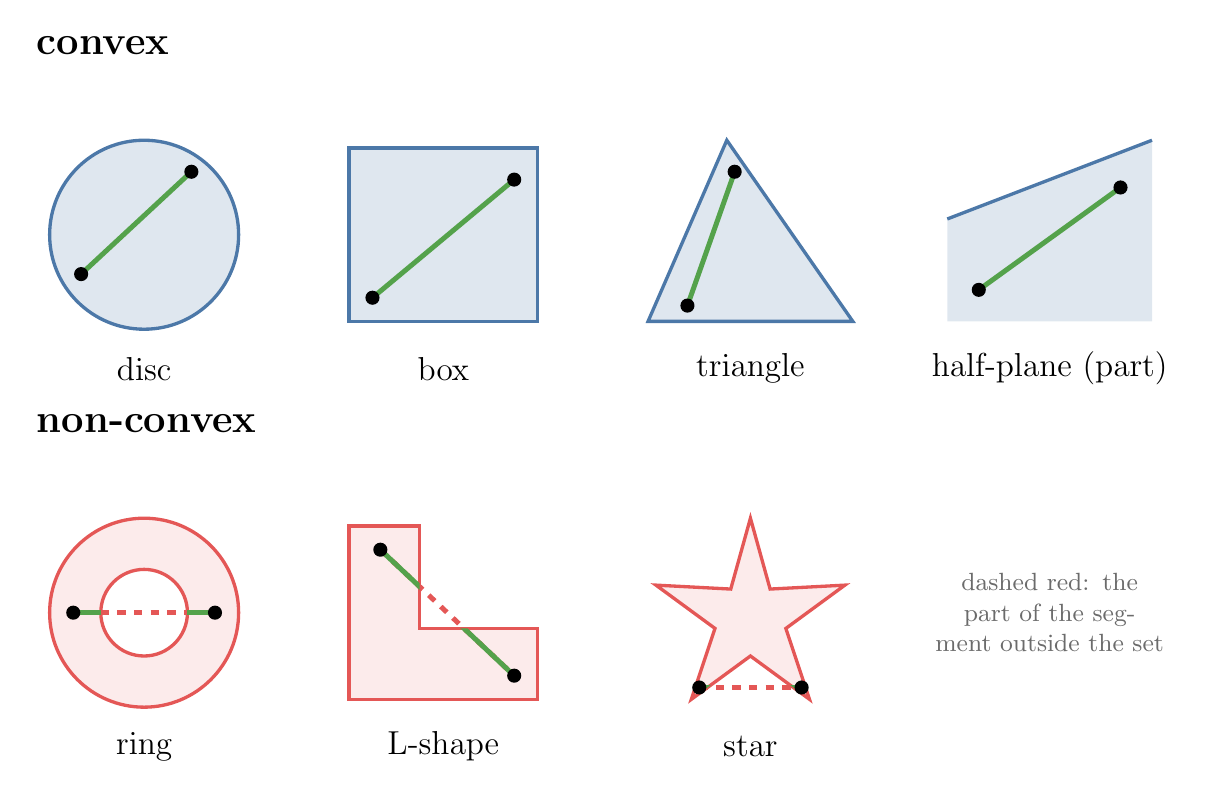
\begin{tikzpicture}[every node/.append style={font=\large}, dot/.style={circle, fill=black, inner sep=1.8pt}]
  % ---------------- top row: convex
  \node[title, anchor=west] at (-1.5,2.4) {convex};
  \fill[cblue!18, draw=cblue] (0,0) circle (1.2);
  \draw[cgreen, line width=1.8pt] (-0.8,-0.5) node[dot]{} -- (0.6,0.8) node[dot]{};
  \node at (0,-1.7) {disc};
  \fill[cblue!18, draw=cblue] (2.6,-1.1) -- (5.0,-1.1) -- (5.0,1.1) -- (2.6,1.1) -- cycle;
  \draw[cgreen, line width=1.8pt] (2.9,-0.8) node[dot]{} -- (4.7,0.7) node[dot]{};
  \node at (3.8,-1.7) {box};
  \fill[cblue!18, draw=cblue] (6.4,-1.1) -- (9.0,-1.1) -- (7.4,1.2) -- cycle;
  \draw[cgreen, line width=1.8pt] (6.9,-0.9) node[dot]{} -- (7.5,0.8) node[dot]{};
  \node at (7.7,-1.7) {triangle};
  \fill[cblue!18] (10.2,-1.1) -- (12.8,-1.1) -- (12.8,1.2) -- (10.2,0.2) -- cycle;
  \draw[cblue] (10.2,0.2) -- (12.8,1.2);
  \draw[cgreen, line width=1.8pt] (10.6,-0.7) node[dot]{} -- (12.4,0.6) node[dot]{};
  \node at (11.5,-1.7) {half-plane (part)};
  % ---------------- bottom row: non-convex
  \begin{scope}[yshift=-4.8cm]
    \node[title, anchor=west] at (-1.5,2.4) {non-convex};
    \fill[cred!12, draw=cred, even odd rule] (0,0) circle (1.2) (0,0) circle (0.55);
    \draw[cgreen, line width=1.8pt] (-0.9,0) node[dot]{} -- (-0.55,0);
    \draw[cred, line width=1.8pt, dashed] (-0.55,0) -- (0.55,0);
    \draw[cgreen, line width=1.8pt] (0.55,0) -- (0.9,0) node[dot]{};
    \node at (0,-1.7) {ring};
    \def\Lshape{(2.6,-1.1) -- (5.0,-1.1) -- (5.0,-0.2) -- (3.5,-0.2) -- (3.5,1.1) -- (2.6,1.1) -- cycle}
    \fill[cred!12, draw=cred] \Lshape;
    \draw[cred, line width=1.8pt, dashed] (3.0,0.8) -- (4.7,-0.8);
    \begin{scope} \clip \Lshape; \draw[cgreen, line width=1.8pt] (3.0,0.8) -- (4.7,-0.8); \end{scope}
    \node[dot] at (3.0,0.8) {}; \node[dot] at (4.7,-0.8) {};
    \node at (3.8,-1.7) {L-shape};
    \def\Star{(7.7,1.2) -- (7.95,0.3) -- (8.9,0.35) -- (8.15,-0.2) -- (8.45,-1.1) -- (7.7,-0.55) -- (6.95,-1.1) -- (7.25,-0.2) -- (6.5,0.35) -- (7.45,0.3) -- cycle}
    \fill[cred!12, draw=cred] \Star;
    \draw[cred, line width=1.8pt, dashed] (7.05,-0.95) -- (8.35,-0.95);
    \begin{scope} \clip \Star; \draw[cgreen, line width=1.8pt] (7.05,-0.95) -- (8.35,-0.95); \end{scope}
    \node[dot] at (7.05,-0.95) {}; \node[dot] at (8.35,-0.95) {};
    \node at (7.7,-1.7) {star};
    \node[note, text width=3.6cm] at (11.5,0) {dashed red: the part of the segment outside the set};
  \end{scope}
\end{tikzpicture}
\end{document}
